\subsection{Overview: high-level components and their interaction}

Since the application is distributed and explicitly designed to support interface between users and the system, the optimal architecture is a client/server one. 

As the system integrates multiple data sources, a three-tier architecture is more adequate. The system is thus divided into a Client Layer, which is the entry point for users, the Business Layer which is embedded in servers, and the Data Layer. 

For sake of simplicity, easiness to install and security, the architecture is designed as a thin client one.

\begin{figure} [!h]
	\centering
	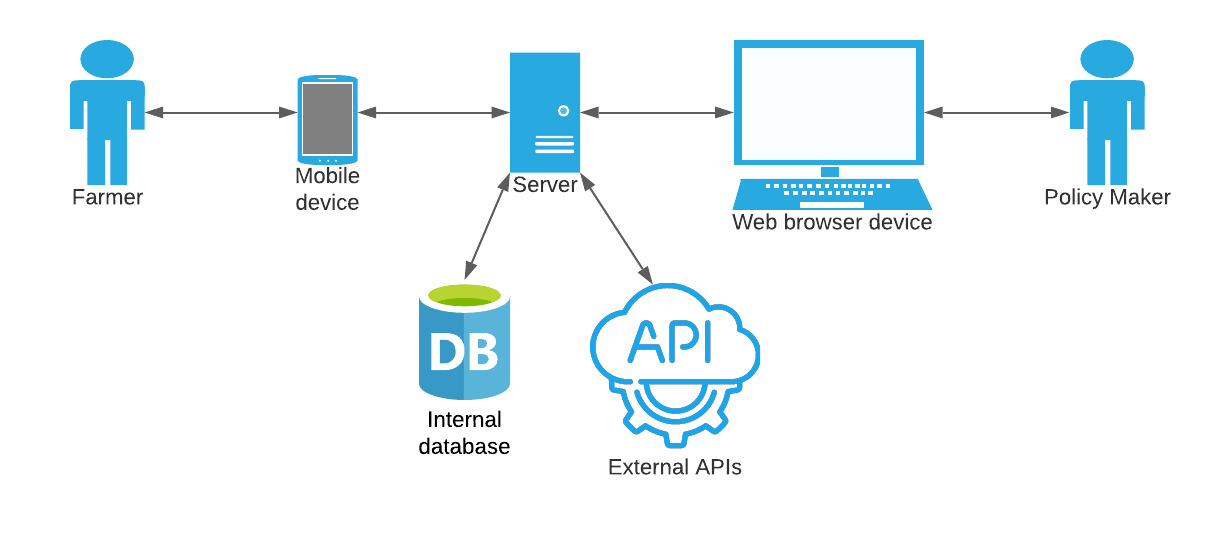
\includegraphics[width=\textwidth]{Images/architecture-diagram.png}
	\caption{\label{fig:seq} Physical architecture diagram}
\end{figure}

\begin{figure} [!h]
	\centering
	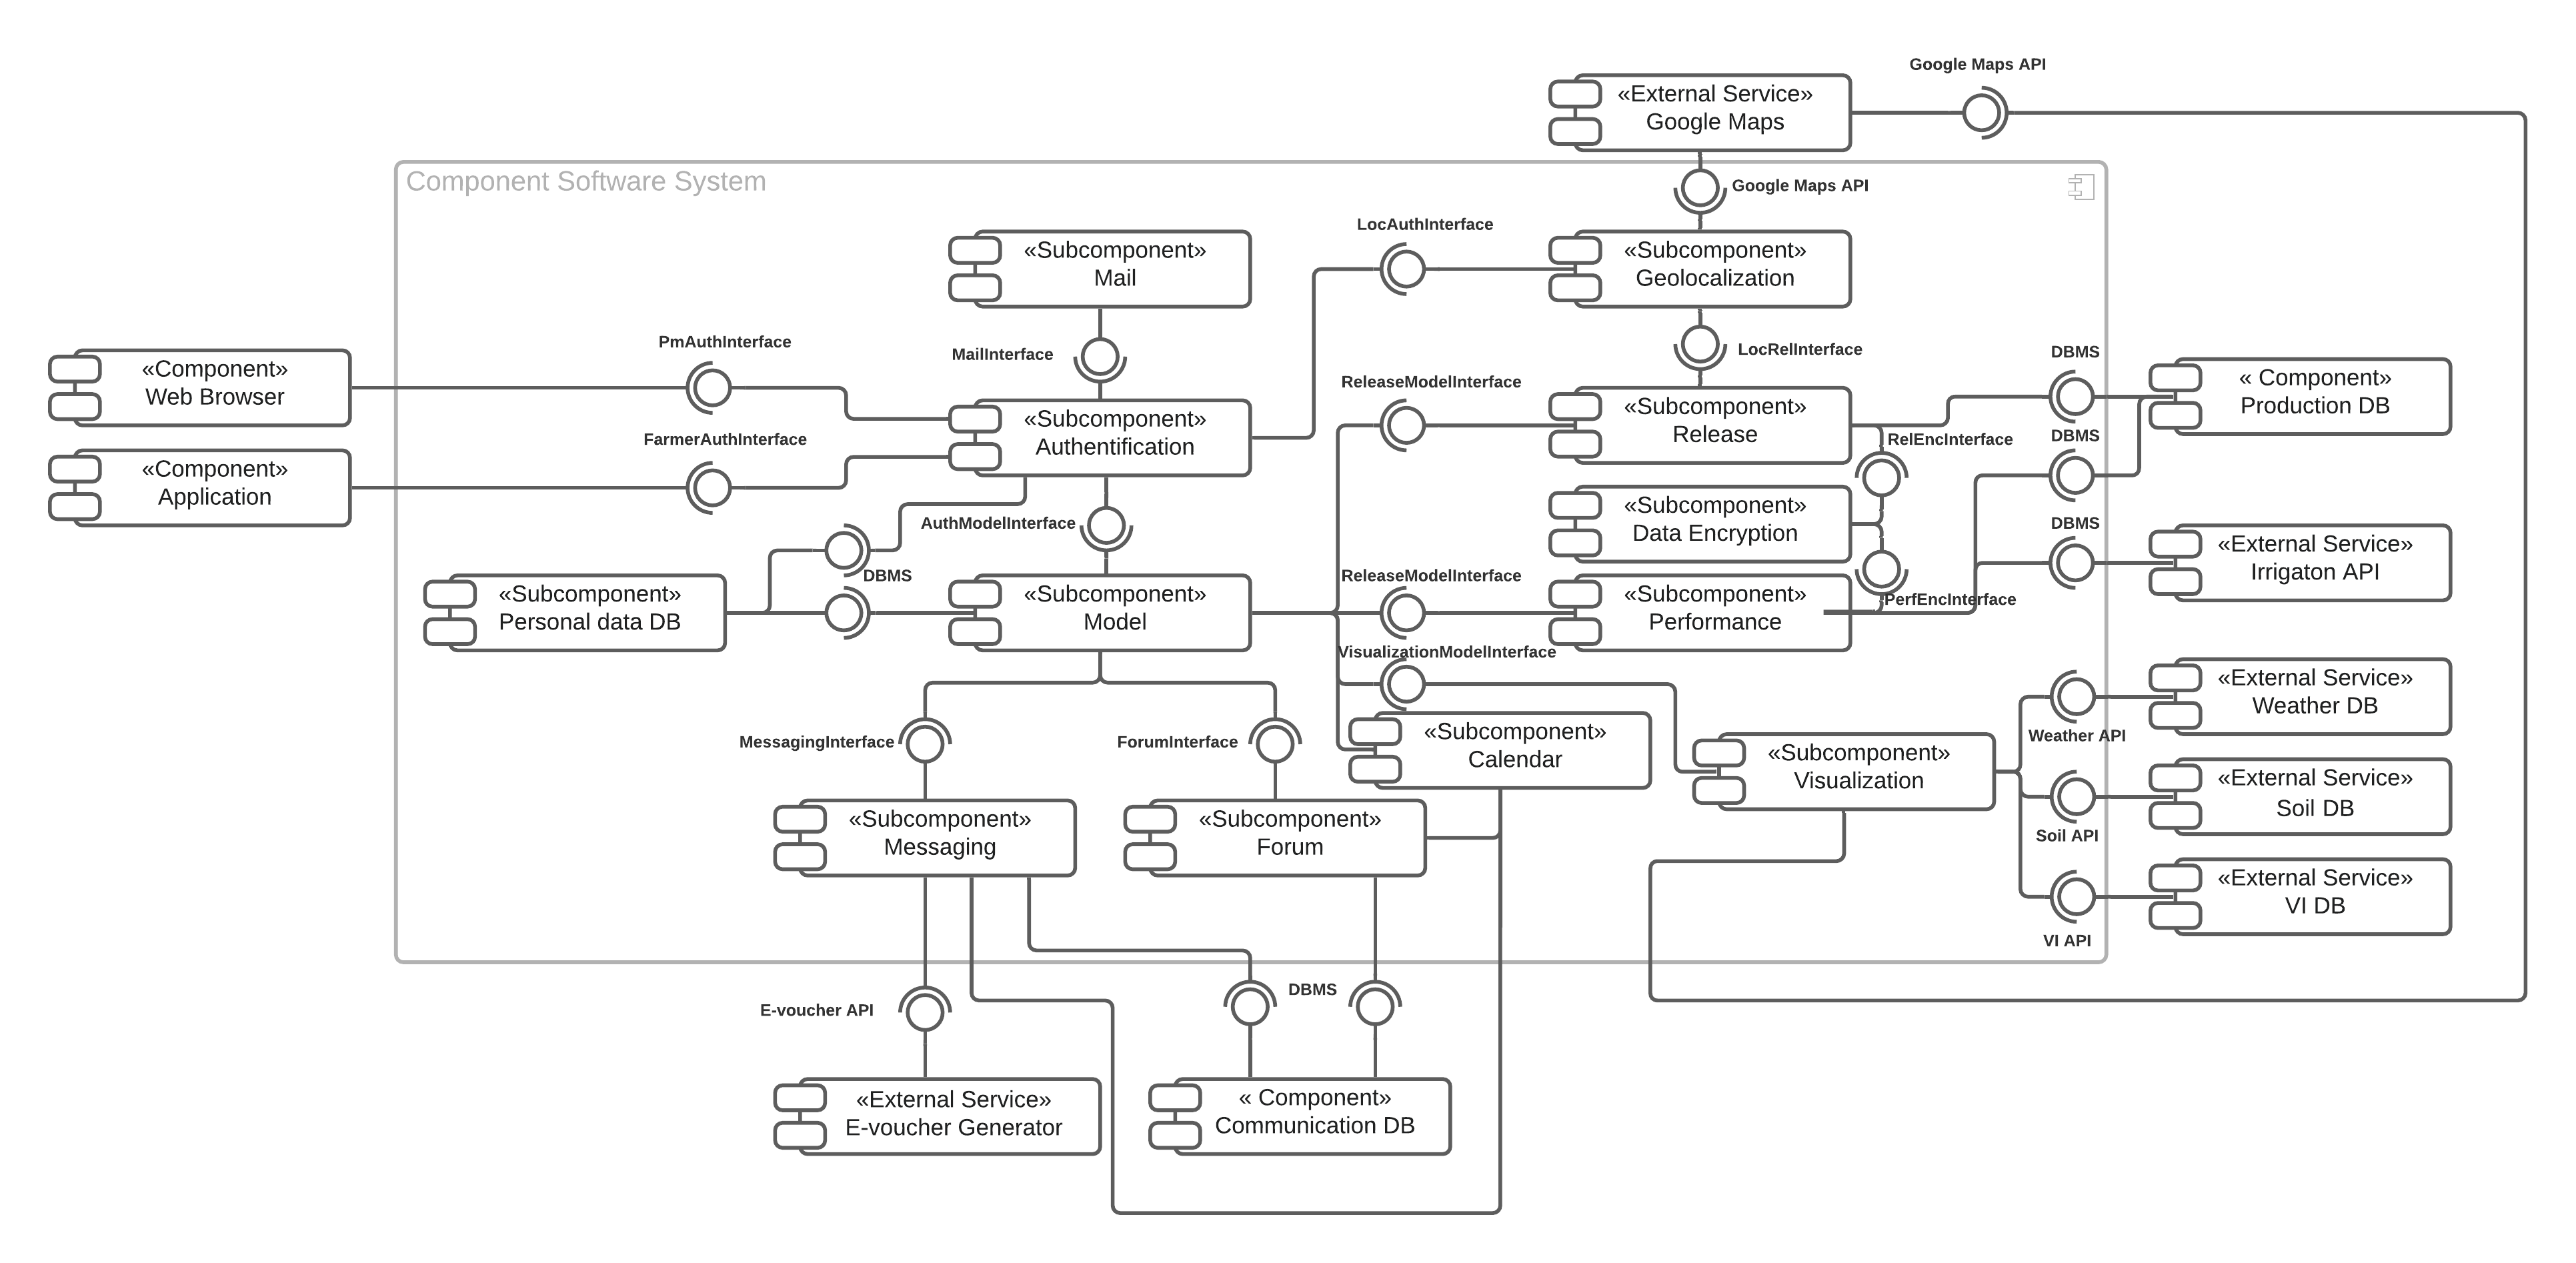
\includegraphics[width=\textwidth]{Images/component-diagram.png}
	\caption{\label{fig:seq} Component diagram}
\end{figure}